%  http://latex-beamer.sourceforge.net/

%\documentclass[landscape]{foils}

%\documentclass{beamer}
%\documentclass[handout]{beamer}     % TO PRINT PRESENTATION HANDOUT
\documentclass[xcolor=dvipsnames]{beamer}  % ALLOWS CHANGE IN COLOR

\usepackage{color}

\usepackage{pifont} %para tener la ballot cross \ding{55}

\usepackage{beamerthemesplit}
\usepackage{url}
\usepackage{ae} % or {zefonts}
\usepackage[T1]{fontenc}
\usepackage[ansinew]{inputenc}
\usepackage[spanish]{babel}

\usepackage{graphicx}
%\graphicspath{"c:/data"}
\usepackage{color}
%\usepackage[colorlinks]{hyperref}
\usepackage{tikz} % Easier syntax to draw pgf files (invokes pgf automatically)
\usetikzlibrary{arrows,shapes.geometric}
%\usepackage{pgfmath} % new version of Tikz loads package automatically


%\usecolortheme{crane}     %Color yellow
%\usetheme{Warsaw}
\usecolortheme[named=Gray]{structure}

\useoutertheme[footline=empty]{}  % PUTS COLORED LINE AT FOOT WITH TITLE, AUTHOR, PAGE, etc
%\usetheme{Berkeley}
\usetheme[height=7mm]{Rochester}
\setbeamertemplate{items}[ball]   % ITEMS IN 3D BALLS (alt CIRCLES)
\setbeamertemplate{navigation symbols}{}  % DROPS NAVIGATION ICONS
\setbeamertemplate{blocks}[rounded][shadow=true]

\usepackage{multirow} %allows multiple rows in tables

%\setbeamertemplate{footline} {
%    \begin{beamercolorbox}{section in head/foot}
%    \insertsectionnavigationhorizontal{\paperwidth}{}{plus1filll
%    \insertframenumber}
%    \end{beamercolorbox}
%}


%\setbeamertemplate{navigation symbols}{\insertslidenavigationsymbol,
%\insertdocnavigationsymbol} \setbeamertemplate{footline} {
%    \begin{beamercolorbox}{section in head/foot}
%    \insertsectionnavigationhorizontal{\paperwidth}{}{plus1filll
%    \insertframenumber}
%    \end{beamercolorbox}
%}

\setbeamercovered{transparent}
\setbeamertemplate{caption}{\insertcaption}

\tikzstyle{nodo} = [circle, draw=black, fill=white, text=black]
\tikzstyle{end} = [circle, minimum width=3pt,fill, inner sep=0pt]

%%\title[Deriva en SCJN]{�Una caja de Pandora?}
%%\subtitle{Activismo y deriva ideol�gica en la Suprema Corte \\ (Resultados *preliminares*)}
%%\author[Magaloni, Magar, S�nchez]{Beatriz Magaloni\inst{1} \and Eric Magar\inst{2} \and Arianna S�nchez\inst{3}}
%%\institute[Stanford, ITAM, Curtis]{ \inst{1}Stanford University \and
%%\inst{2}ITAM \and \inst{3}Curtis, Mallet-Prevost, Colt Mosle LLP,
%%New York}
%%\date[26may10]{26 de mayo 2010}

\begin{document}

%%%%%%%%%%%%%%%%%%%%%%%%%%%%%%%%%%%%%%%%%%%%%%%%%%%%%%%%%%%%%%%%%%%%%%%%%%%%%%%%%%%%%%%%%%%%

%\frame[plain]{\titlepage}

%%%%%%%%%%%%%%%%%%%%%%%%%%%%%%%%%%%%%%%%%%%%%%%%%%%%%%%%%%%%%%%%%%%%%%%%%%%%%%%%%%%%%%%%%%%%

\frame {                      % SLIDE

    \frametitle{Puntos ideales, $IV^a$ Legislatura de la ALDF}

\tiny{Lo que a continuaci�n aparece son resultados preliminares de un an�lisis de votaciones nominales divididas en la ALDF que estamos realizando Eric Magar, Mariel Melka y Rafael Ch. Cubre la cuarta Legislatura (2006-09), pero las estimaciones de puntos ideales s�lo llegan hasta el primer cuadrimestre 2009 (posteriormente no hubo votaciones divididas).

Para interpretar el espacio bidimensional en el que estimamos el punto ideal de cada legislador, hay que tomar en cuenta que fijamos arbitrariamente los par�metros del modelo de la siguiente manera. Les corresponde a ustedes interpretar la sustancia que subyace al espacio abstracto. Me referir� por ahora a las coordenadas norte, sur, este y oeste del espacio.

%(Nota EMM: esta interpretaci�n es v�lida para los resultados post-rotaci�n de 45 grados; tendr� que verificar que obtengo algo similar con priors S-E-O en vez de SO-NE-SE).

\bigskip

\begin{tabular}{cccc}
    Id & Fecha & ``Cleavage'' / asunto & Votar a favor implica un punto ideal al \\ \hline
    V1 & 09/11/06 & Vertical / Sociedades de convivencia & oeste \\
    H1 & 26/12/06 & Horizontal / Designaci�n 5 magistrados electorales & sur \\
    V2 & 28/12/06 & Vertical / L�nea de cr�dito proyecto ley de egresos & este \\
    H2 & 29/05/08 & Horizontal / Ratificaci�n consejeros IEDF & sur \\
\end{tabular}

\bigskip

En el sitio web de la asamblea (\url{http://www.aldf.gob.mx/diario-debates-204-1.html}) podr�n consultar el diario de debates. Les permitir� reconstruir lo ocurrido en �sas y otras sesiones (el diario incluye el resultado de las votaciones nominales).

El archivo aldfIdPts.xls anexo contiene las coordenadas en los ejes X y Y de cada legislador para cada cuadrimestre.

}

}

%%%%%%%%%%%%%%%%%%%%%%%%%%%%%%%%%%%%%%%%%%%%%%%%%%%%%%%%%%%%%%%%%%%%%%%%%%%%%%%%%%%%%%%%%%%%

\frame {                      % SLIDE

    \frametitle{Cuatrimestre 2006--3~~~~($t=1$)}

\begin{center}
\begin{tabular}{c}
   \includegraphics[width=8.25cm]{2006-3.pdf}
%   \includegraphics[width=8.25cm]{d:/01/data/rollcall/aldf/graphs/2006-3.pdf}
\end{tabular}
\end{center}

}

\end{document}

%%%%%%%%%%%%%%%%%%%%%%%%%%%%%%%%%%%%%%%%%%%%%%%%%%%%%%%%%%%%%%%%%%%%%%%%%%%%%%%%%%%%%%%%%%%%

\frame {                      % SLIDE

    \frametitle{Cuatrimestre 2007--1~~~~($t=2$)}

\begin{center}
\begin{tabular}{c}
   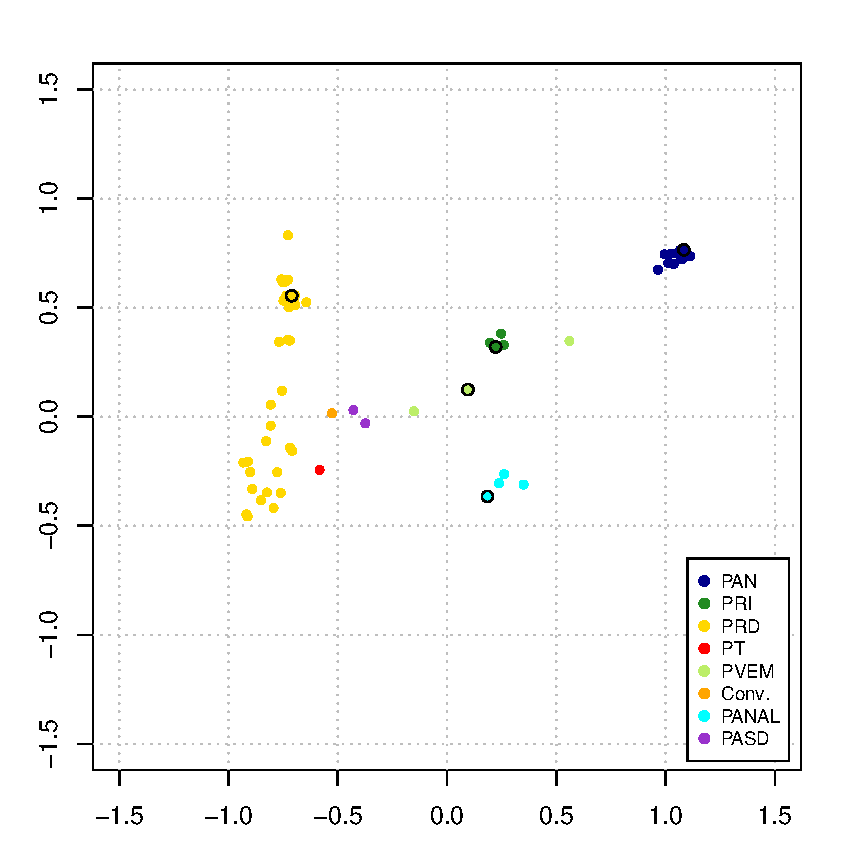
\includegraphics[width=8.25cm]{d:/01/data/rollcall/aldf/graphs/2007-1.pdf}
\end{tabular}
\end{center}

}

%%%%%%%%%%%%%%%%%%%%%%%%%%%%%%%%%%%%%%%%%%%%%%%%%%%%%%%%%%%%%%%%%%%%%%%%%%%%%%%%%%%%%%%%%%%%

\frame {                      % SLIDE

    \frametitle{Cuatrimestre 2007--2~~~~($t=3$)}

\begin{center}
\begin{tabular}{c}
   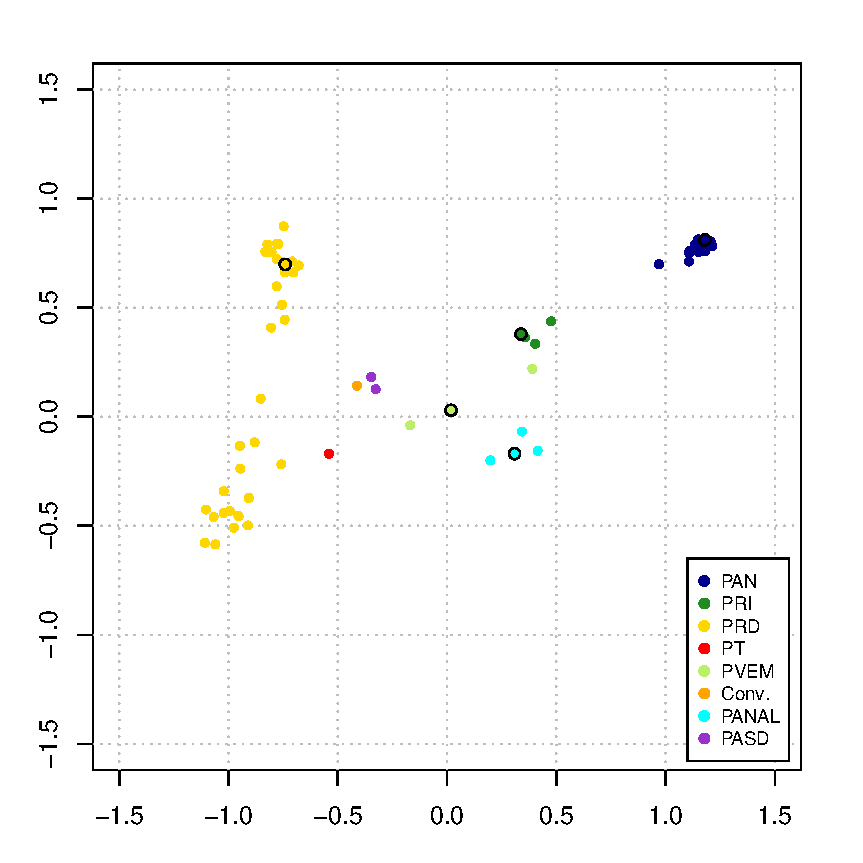
\includegraphics[width=8.25cm]{d:/01/data/rollcall/aldf/graphs/2007-2.pdf}
\end{tabular}
\end{center}

}

%%%%%%%%%%%%%%%%%%%%%%%%%%%%%%%%%%%%%%%%%%%%%%%%%%%%%%%%%%%%%%%%%%%%%%%%%%%%%%%%%%%%%%%%%%%%

\frame {                      % SLIDE

    \frametitle{Cuatrimestre 2007--3~~~~($t=4$)}

\begin{center}
\begin{tabular}{c}
   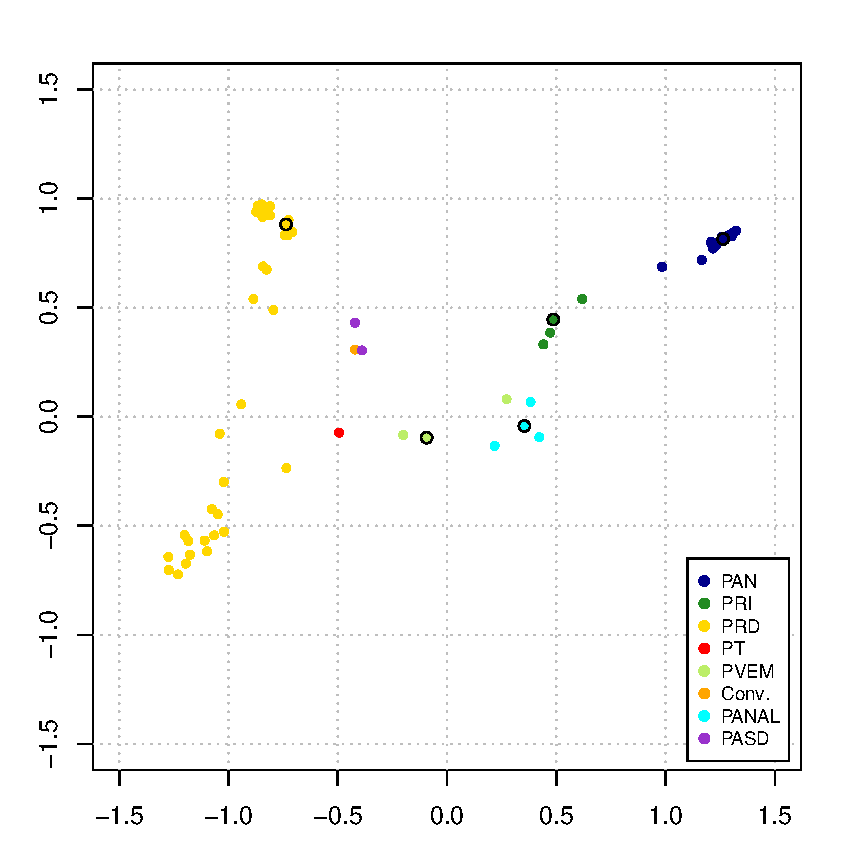
\includegraphics[width=8.25cm]{d:/01/data/rollcall/aldf/graphs/2007-3.pdf}
\end{tabular}
\end{center}

}

%%%%%%%%%%%%%%%%%%%%%%%%%%%%%%%%%%%%%%%%%%%%%%%%%%%%%%%%%%%%%%%%%%%%%%%%%%%%%%%%%%%%%%%%%%%%

\frame {                      % SLIDE

    \frametitle{Cuatrimestre 2008--1~~~~($t=5$)}

\begin{center}
\begin{tabular}{c}
   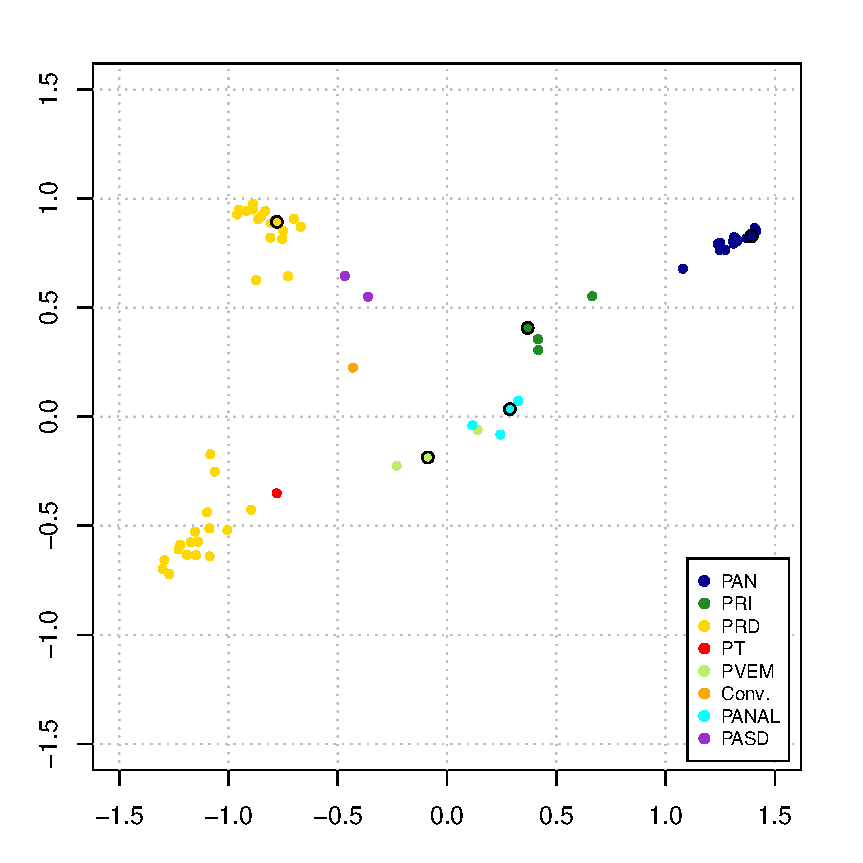
\includegraphics[width=8.25cm]{d:/01/data/rollcall/aldf/graphs/2008-1.pdf}
\end{tabular}
\end{center}

}

%%%%%%%%%%%%%%%%%%%%%%%%%%%%%%%%%%%%%%%%%%%%%%%%%%%%%%%%%%%%%%%%%%%%%%%%%%%%%%%%%%%%%%%%%%%%

\frame {                      % SLIDE

    \frametitle{Cuatrimestre 2008--2~~~~($t=6$)}

\begin{center}
\begin{tabular}{c}
   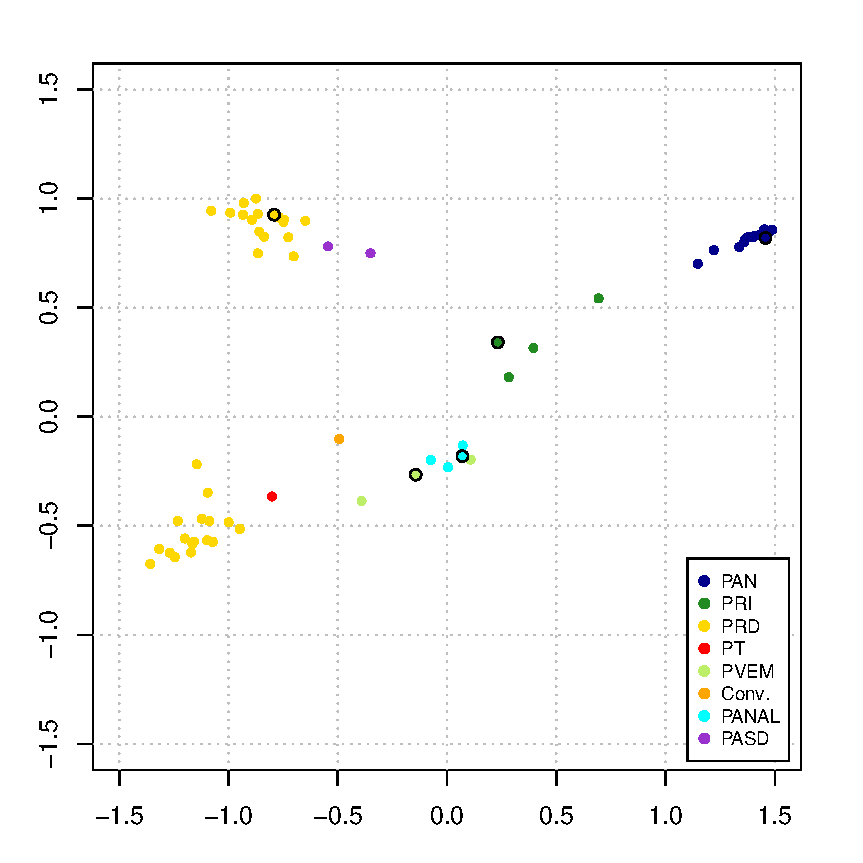
\includegraphics[width=8.25cm]{d:/01/data/rollcall/aldf/graphs/2008-2.pdf}
\end{tabular}
\end{center}

}

%%%%%%%%%%%%%%%%%%%%%%%%%%%%%%%%%%%%%%%%%%%%%%%%%%%%%%%%%%%%%%%%%%%%%%%%%%%%%%%%%%%%%%%%%%%%

\frame {                      % SLIDE

    \frametitle{Cuatrimestre 2008--3~~~~($t=7$)}

\begin{center}
\begin{tabular}{c}
   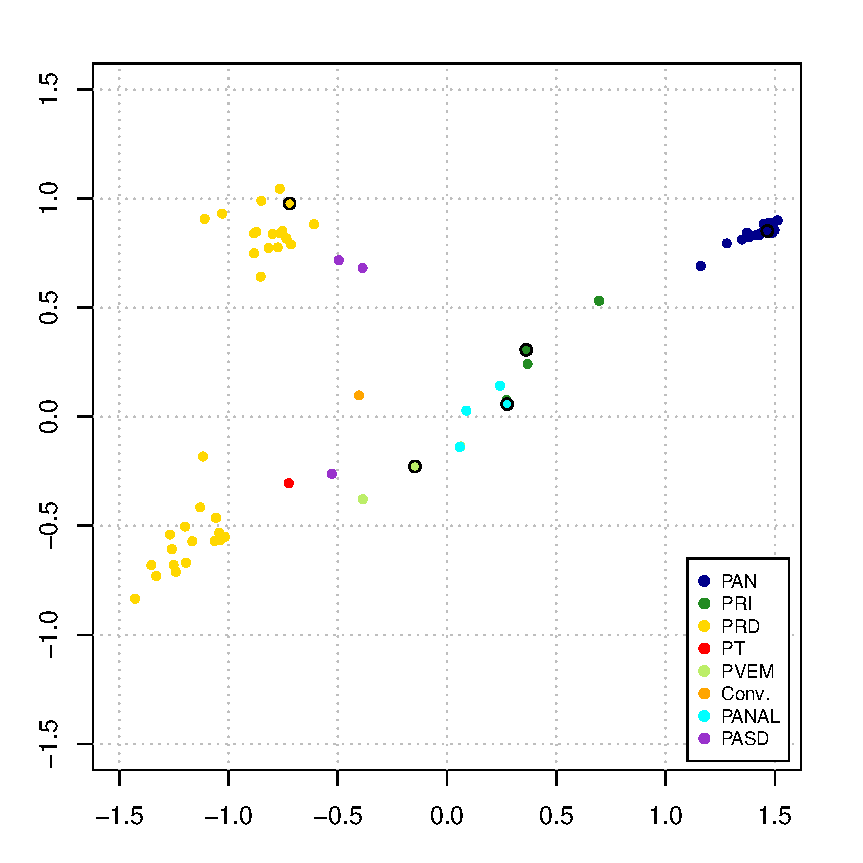
\includegraphics[width=8.25cm]{d:/01/data/rollcall/aldf/graphs/2008-3.pdf}
\end{tabular}
\end{center}

}

%%%%%%%%%%%%%%%%%%%%%%%%%%%%%%%%%%%%%%%%%%%%%%%%%%%%%%%%%%%%%%%%%%%%%%%%%%%%%%%%%%%%%%%%%%%%

\frame {                      % SLIDE

    \frametitle{Cuatrimestre 2009--1~~~~($t=8$)}

\begin{center}
\begin{tabular}{c}
   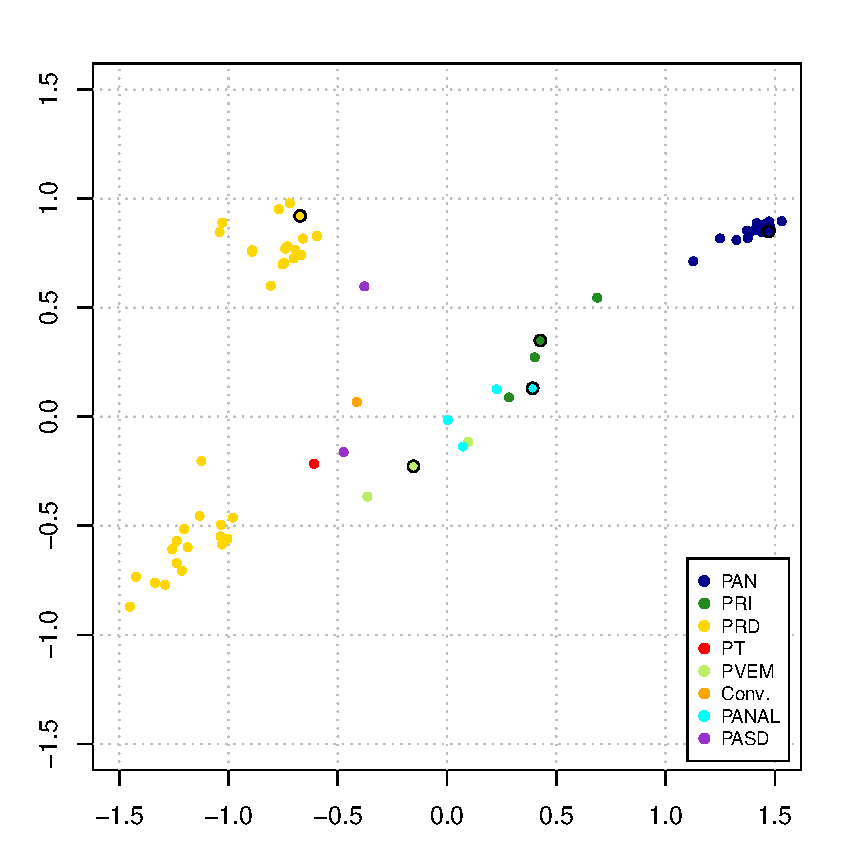
\includegraphics[width=8.25cm]{d:/01/data/rollcall/aldf/graphs/2009-1.pdf}
\end{tabular}
\end{center}

}

%%%%%%%%%%%%%%%%%%%%%%%%%%%%%%%%%%%%%%%%%%%%%%%%%%%%%%%%%%%%%%%%%%%%%%%%%%%%%%%%%%%%%%%%%%%%

\frame {                      % SLIDE

    \frametitle{Los ``cutlines'' estimados}

\begin{center}
\begin{tabular}{cccc}
    2006--3 & 2007--1 & 2007--2 & 2007--3 \\
   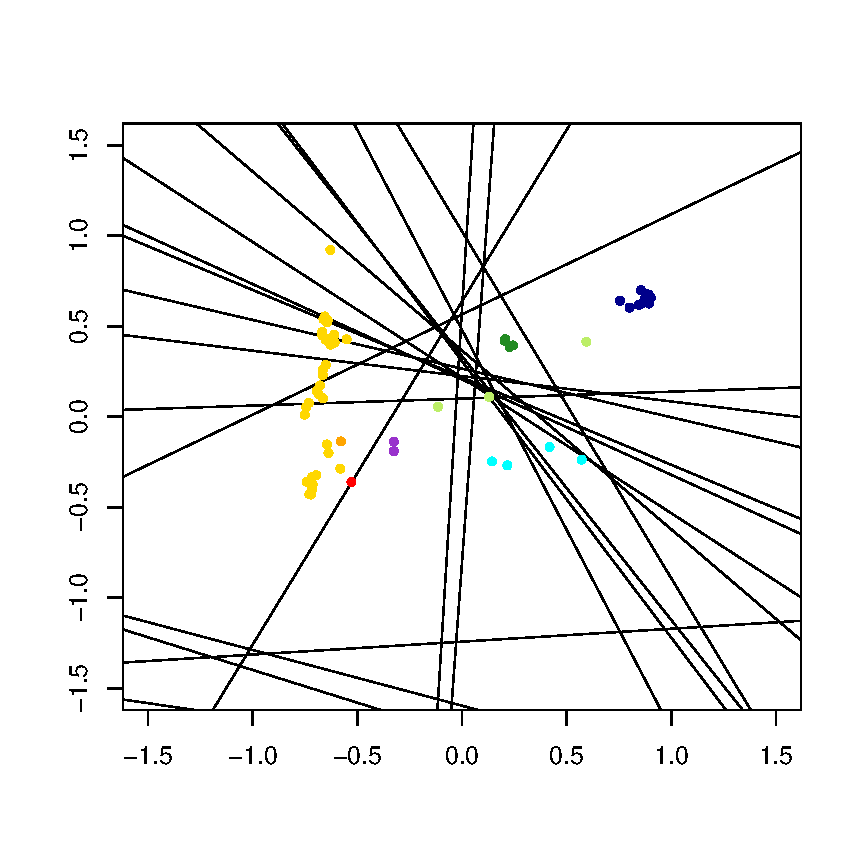
\includegraphics[width=2.5cm]{d:/01/data/rollcall/aldf/graphs/2006-3cutlines.pdf} &
   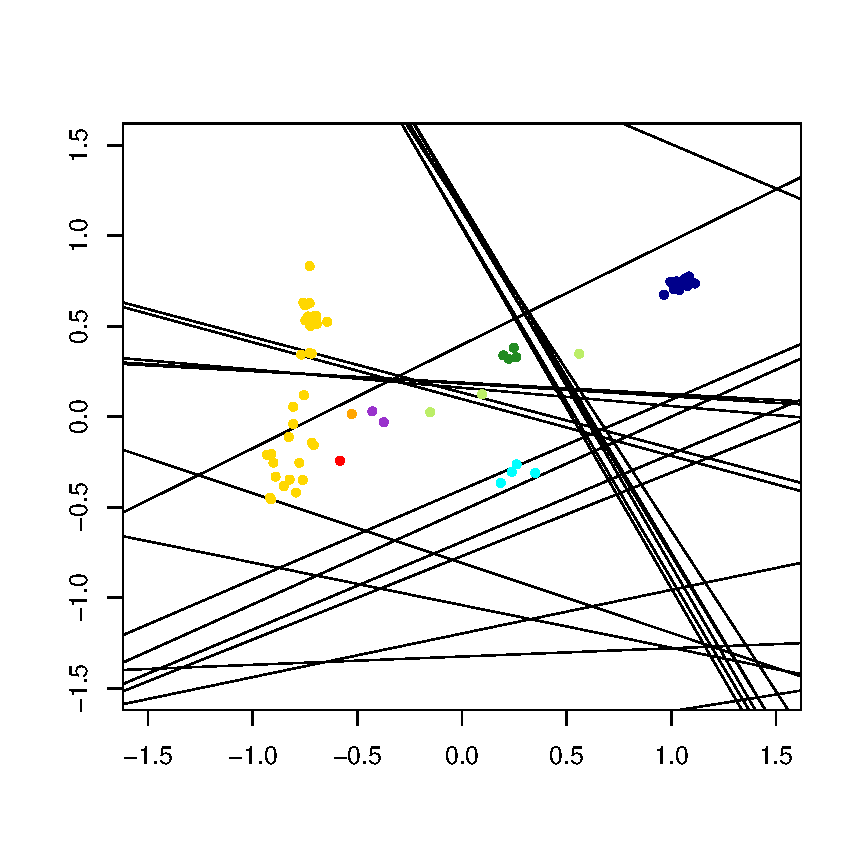
\includegraphics[width=2.5cm]{d:/01/data/rollcall/aldf/graphs/2007-1cutlines.pdf} &
   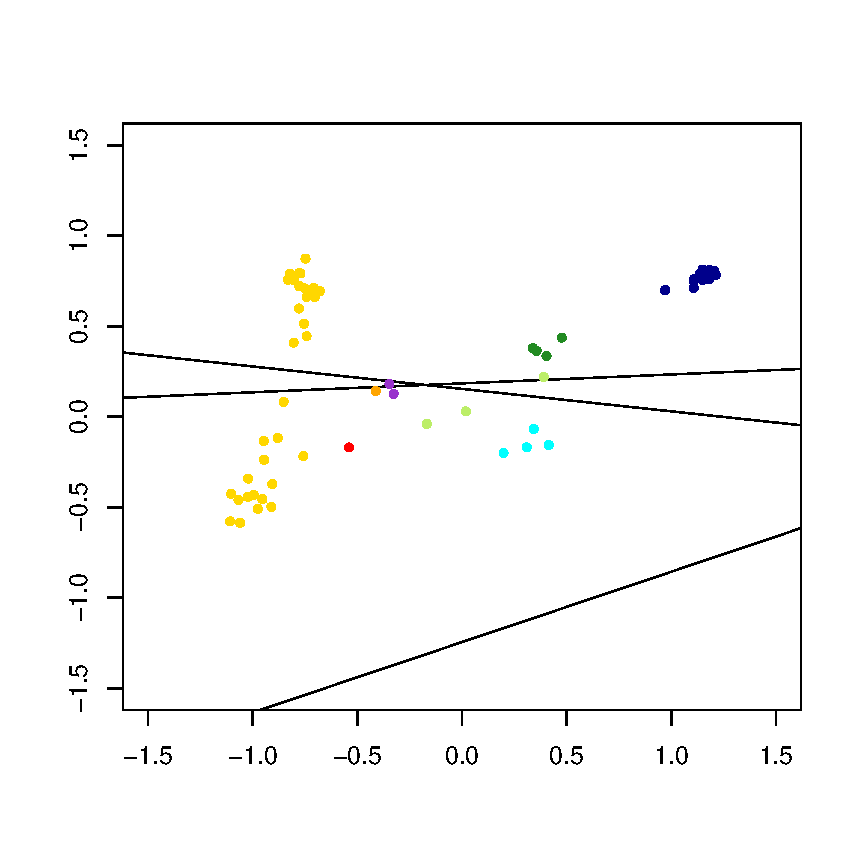
\includegraphics[width=2.5cm]{d:/01/data/rollcall/aldf/graphs/2007-2cutlines.pdf} &
   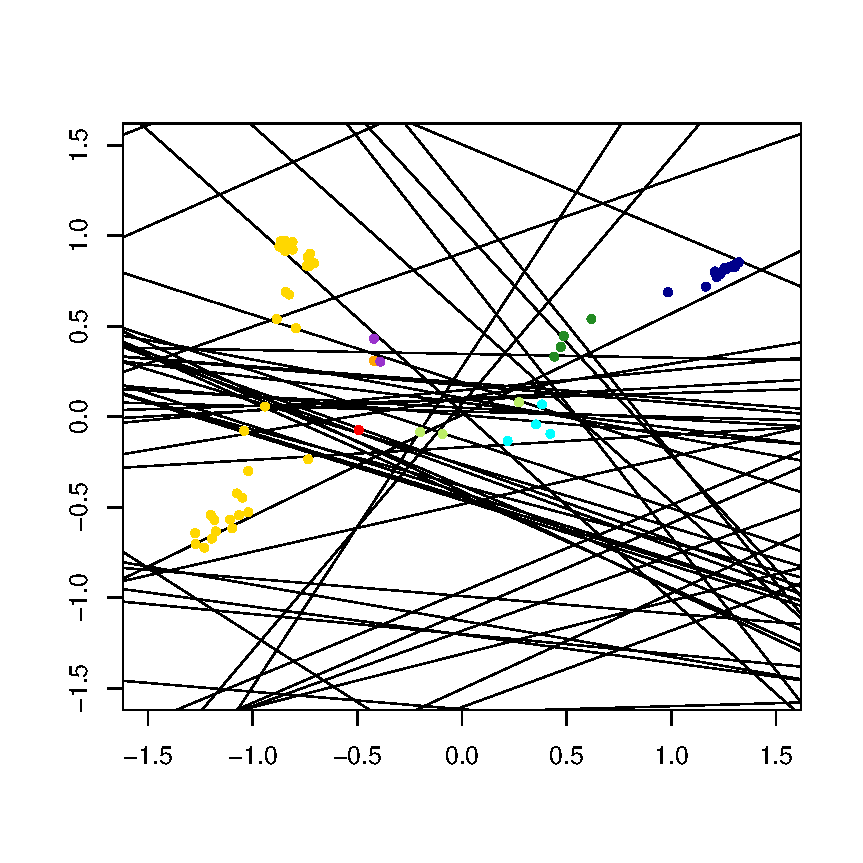
\includegraphics[width=2.5cm]{d:/01/data/rollcall/aldf/graphs/2007-3cutlines.pdf} \\
    2008--1 & 2008--2 & 2008--3 & 2009--1 \\
   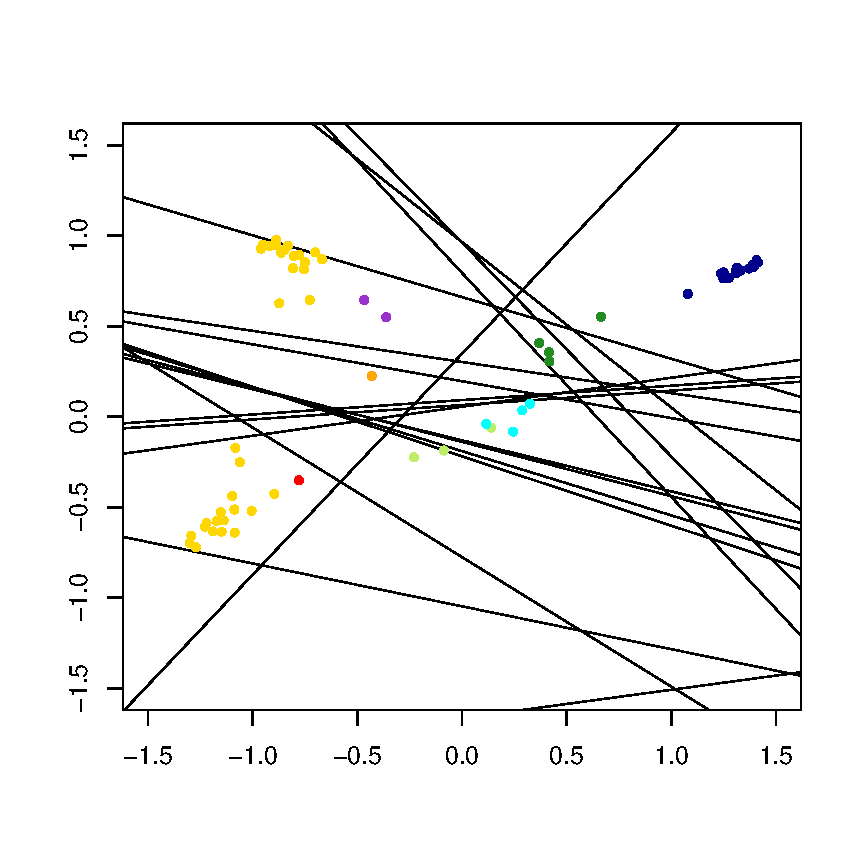
\includegraphics[width=2.5cm]{d:/01/data/rollcall/aldf/graphs/2008-1cutlines.pdf} &
   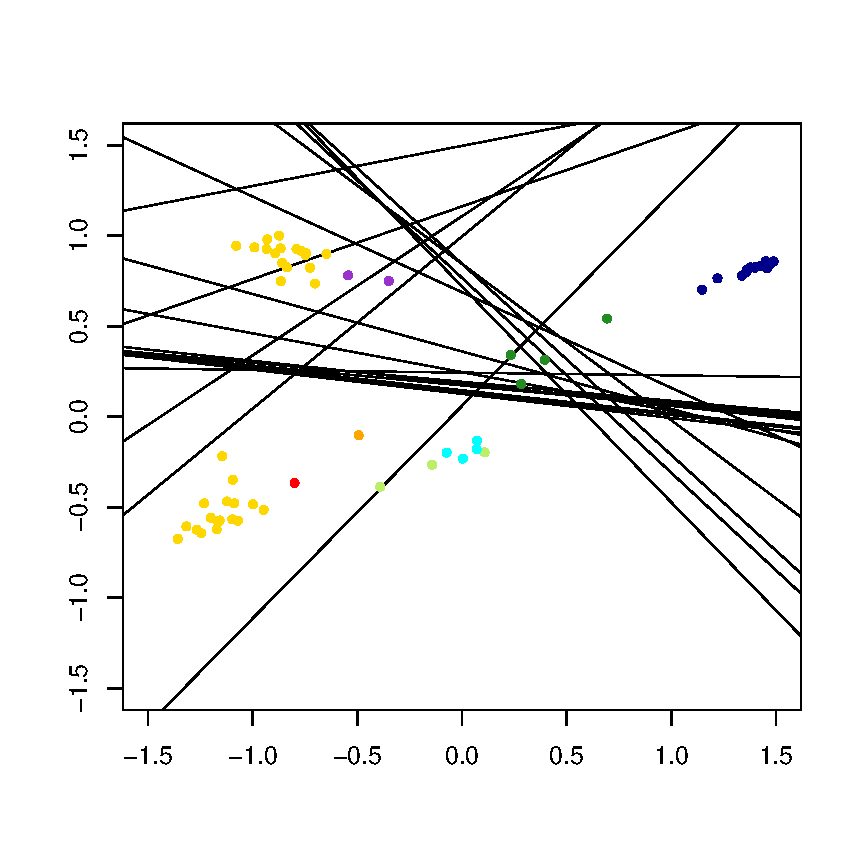
\includegraphics[width=2.5cm]{d:/01/data/rollcall/aldf/graphs/2008-2cutlines.pdf} &
   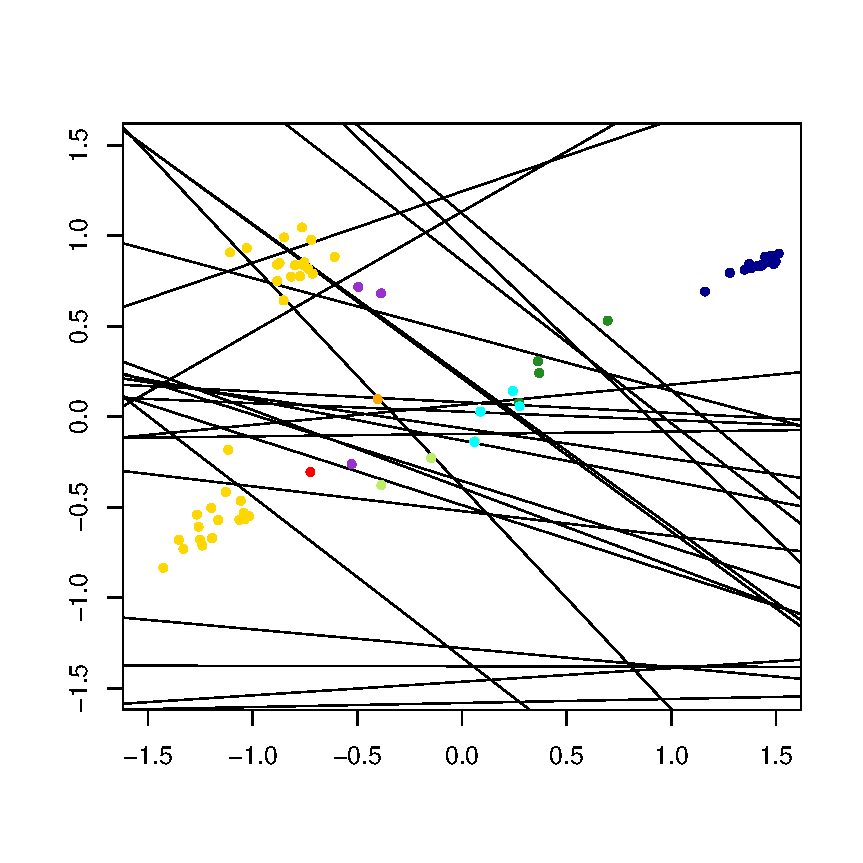
\includegraphics[width=2.5cm]{d:/01/data/rollcall/aldf/graphs/2008-3cutlines.pdf} &
   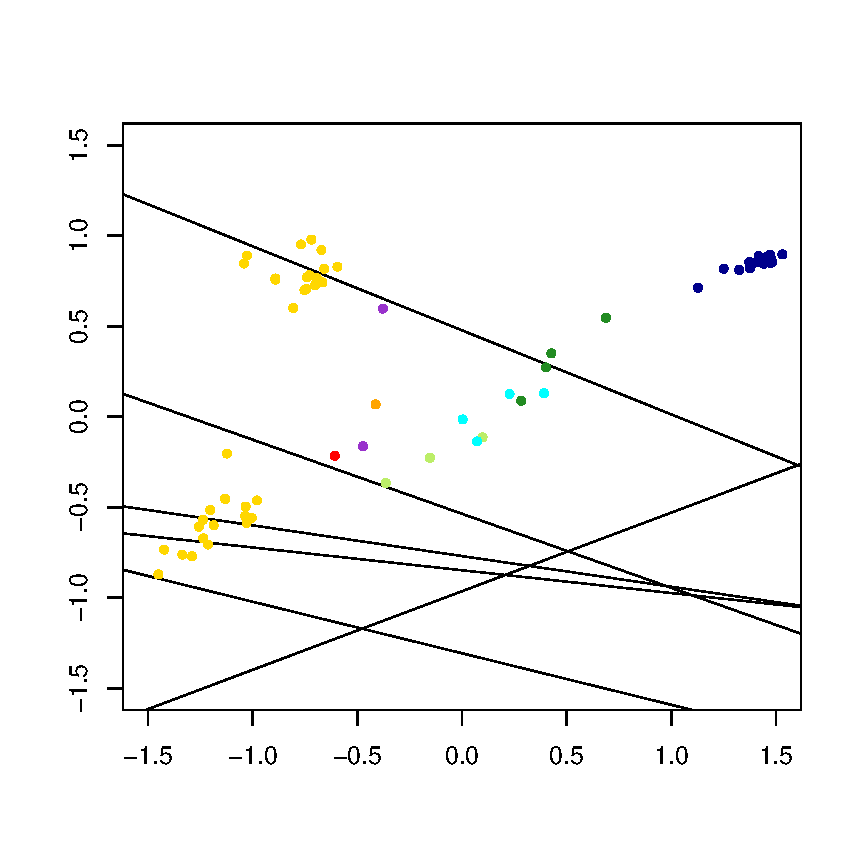
\includegraphics[width=2.5cm]{d:/01/data/rollcall/aldf/graphs/2009-1cutlines.pdf} \\
\end{tabular}
\end{center}

}
\end{document}
